% This is a template for doing homework assignments in LaTeX
% !TeX TXS-program:bibliography = txs:///biber
\documentclass{article} % This command is used to set the type of document you are working on such as an article, book, or presenation

\usepackage[margin=0.5in]{geometry} % This package allows the editing of the page layout
\usepackage{amsmath}  % This package allows the use of a large range of mathematical formula, commands, and symbols
\usepackage{graphicx}  % This package allows the importing of images
\usepackage{algorithm2e}
\usepackage{amsfonts} 
\usepackage{graphicx}
\usepackage{makecell}
\usepackage{verbatim}
\usepackage{mathtools}
\usepackage{subcaption}
\usepackage[nottoc]{tocbibind}
\title{\vspace{-2cm}How much data do you need? Predicting class specific training dataset sizes.}
\author{Thomas Mühlenstädt}
\date{\vspace{-5ex}}
\graphicspath{ {./plots/} }
\RestyleAlgo{ruled}

%
\newcommand{\nosemic}{\SetEndCharOfAlgoLine{\relax}}% Drop semi-colon ;
\newcommand{\dosemic}{\SetEndCharOfAlgoLine{\string;}}% Reinstate
\newcommand{\pushline}{\Indp}% Indent
\newcommand{\popline}{\Indm\dosemic}% Undent
%

\begin{document}
\maketitle


\subsection*{Introduction}

This paper targets the question of predicting machine learning classification model performance, when taking into account the number of training examples per class and not just the overall number of training examples.
This leads to the a combinatorial question, which combinations of number of training examples per class should be considered, given a fixed overall training dataset size. 
In order to solve this question, an algorithm is suggested which is motivated from special cases of space filling design of experiments.
The resulting data are modeled using models like powerlaw curves, extended like generalized linear models. While there exist many methods 
in literature dealing with the topic of predicting neural network performance based on training dataset size (see e.g. \cite{hestness2017deep}, \cite{cho2016data}, 
\cite{hoffmann2022training} and \cite{alabdulmohsin2022revisiting}) to the best of our knowledge, this is the first time, that individual class counts per training data set are considered as well. 
This paper is a summary of \cite{muehlenstaedt2024data}.

\subsection*{Method overview}

The task considered in this paper is image classification.
The training data consists of $k$ classes, with each class $j$ having $n_k^{max}$ labeled images in the training dataset with $n^{max} = n_k^{max}$ being the overall 
number of training images, assuming equal number of training images per class.
For completeness, we assume there is a labelled test data set available to calculate the accuracy (or other metrics) of a trained model $f_{\hat{\theta}}(x)$.
Most of the literature for neural scaling laws focusses on assuming different training dataset sizes $n^{train} <= n^{max}$ for a number of different training jobs, i.e. to find a function $g_{\omega}(n^{train})$ which predicts the chosen performance metric for different training dataset sizes.
This means implicitly that each class has the same importance for the performance.
However, this is not necessarily true, some classes might be more difficult to train on than others.
We expand the function $g_{\omega}(n^{train})$ to be more general:  $g_{\omega}(n_1^{train}, \dots, n_k^{train}, n^{epoch})$ shall be a function predicting the performance of our model depending on the individual class training image counts as well as the number of epochs trained on.
In order to fit functions like $g_{\omega}(n_1^{train}, \dots, n_k^{train}, n^{epoch})$ more divers training datasets need to be generated.

\subsection*{Data generation algorithm}

A first idea for sampling datasets could be to assign equal probabilities for selection to each image and to sample a number of times. However, due to the law of large numbers, 
this would result in datasets which are very similar ot each other w.r.t the class distributions. 
In order to achieve a number of more divers training datasets, both with respect to the total size as well with respect to the class proportions, an algorithm is suggested in the following.
It takes motivation from a special case of statistical design of experiments, notably constrained space filling mixture designs  \cite{gomes_hal_spacefilling_mixtures}, which aim at constructing compositions 
of ingredients for chemical experiments, \cite{Nist_2012_eng_stats}, chapter 5.5.4. 

Given a target dataset size $n_{subset}$, we want to create a number of different combinations of training datasets, which all 
have the same total number of training images but distributed differently among to the different classes.
The algorithm to find an optimal design has 2 stages. First, in the initialization phase, a design is constructed which is fullfilling that 
each experiment row is summing up to $n_{subset}$ and the constraint for the maximum number of images per class is fullfilled.
In the second stage, this design is improved iteratively by a pointwise exchange algorithm: The pair of design points with the minimal distance is found and one of them is 
replaced by a new, randomly generated candidate design point, which aims at improving the so called maximin design criterion.
If the maximin criterion for the new candidate design is improved compared to the previously best design, the candidate design is accepted as new best design.
Otherwise, the candidate design is rejected. This process is repeated a fixed number of times. Similar pointwise optimization procedures are frequently applied in design experiments \cite{fedorov1972theory}.
The same process is repeated for different number of subset sizes.

\subsection*{Scaling law model fitting}

So far the standard way of fitting a model to the data is a non-linear least squares fit with different types of underlying model equations, all depending on the overall training dataset size $n$.
Non-linear least squares are implemented in the scipy function \verb|curve_fit| \cite{2020SciPy}.
The power law scaling \cite{mahmood2022data} is a frequently chosen option: $g_{\omega}(n) = \omega_1 n^{\omega_2} + \omega_3$.
But also arctan scaling ($g_{\omega}(n) = \frac{200}{\pi} \arctan(\omega_1 \frac{\pi}{2}n + \omega_2) + \omega_3$),
logarithmic scaling ($g_{\omega}(n) = \omega_1 \log(n + \omega_2) + \omega_3$) and
algebraic root ($g_{\omega}(n) = \frac{100n}{1 + \| \omega_1 n\|^{1/\omega_2}} + \omega_3$) are possible choices.
For each of these models, we can replace $n$ by a linear combination of $n_c$ with a parameter $\beta_c$: $\sum_{c = 1}^C \beta_c n_c$.
Another modification which is done here is to use a combination of different modelling functions, specifically a combination of the powerlaw model and an arctan model.
Also, as the modifications introduced above might result in a high number of model effects for datasets with many classes, methods like forward selection can be applied to avoid having models with a high number of parameters.

\subsection*{Experiment setup with CIFAR10}

The CIFAR10 dataset \cite{Cifar10} is a well known benchmark dataset for image classification.
It consists of 50000 training images, in 10 classes and 10000 test images of the same shape.
A standard Resnet18 architecture \cite{he2015resnet} is used for classification as implemented in the pytorch \cite{pytorch} model zoo using a standard SGD optimizer with cross entropy loss.
With these settings, validation dataset accuracies up to 84\% are achieved.
For the experiments done here, we applied the suggested algorithm with the following settings:
As subset sizes we have chosen $[5000, 10000, \dots, 40000, 45000]$. For each subset size a design of experiments with 30 different settings has been created for training a function $g_{\omega}$ as well as a validation dataset with 15 runs per subset size, training up to 195 epochs.

To get an impression of the models fitted here, there are a number of descriptive visualizations in Figure 
\ref{fig:desc_plots_cifar10}, showing accuracy over epochs for the full training dataset (left), the distribution of test accuracies over training dataset sizes (middle) and as an example 
the test accuracy over epoch for the training dataset size $= 30000$.
 Overall, the descriptive analysis did not yield any concerns in terms of outliers or unexpected behavior of the data.

\subsection*{Model fitting results}
A number of different models are fitted, all using the above described dataset. In Table \ref{table:cifar_model_overview} an overview of the fitted models is given, always using a power law model with different linear combinations.
Model $(0)$ is easily motivated by the idea of generalized linear models \cite{GeneralizedLinearModels}.
However when analyzing the modeling results for this model the prediction plots still looked like containing some signal in the dataset is not captured by the fitted powerlaw model.
This motivated model $(1)$: 
A class count can have a very strong or weak overall maximum effect to the response fitted, and an input can actually achieve it's maximum effect with either very small or only very high counts.
This is achieved by the 2-parameter arctan effect $\beta_{., 1} \arctan{(\beta_{., 2} x)}$. The $\beta_{.,1}$ parameter describes the maximum possible influence of an input 
and the $\beta_{., 2}$ describes the necessary size/counts of input $x$ to achieve this maximum influence.
A standard powerlaw model $(2)$ has been fitted, using total training dataset size and the number of epochs.
In order to have a fair comparison, model $(3)$ is fitted, which is using the same 2-parameter arctan effect as in model $(1)$.

\begin{figure}
    \begin{subfigure}{.3\textwidth}
        \centering
        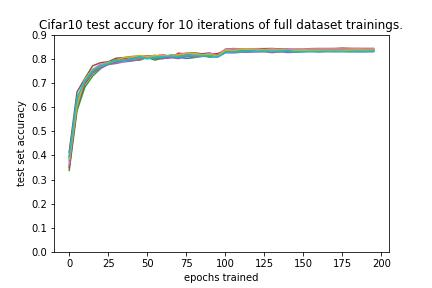
\includegraphics[width=.8\linewidth]{cifar10/Cifar10_full_dataset_acc_vs_epoch.jpg}
        \caption{Full training results for 10 separate training runs.}
        \label{fig_full_dataset_epoch_vs_acc_cifar}
    \end{subfigure}%
    \begin{subfigure}{.3\textwidth}
        \centering
        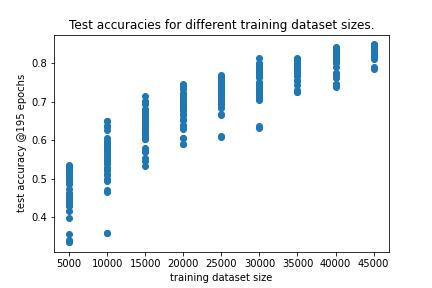
\includegraphics[width=.8\linewidth]{cifar10/Cifar10_training_datasetsize_vs_test_acc.jpg}
        \caption{Test accuracies vs. training dataset sizes.}
        \label{fig_traing_subset_size_vs_test_acc_cifar}
    \end{subfigure}
    \begin{subfigure}{.3\textwidth}
        \centering
        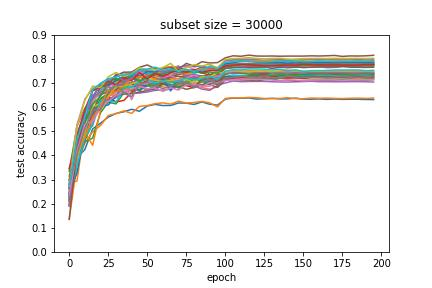
\includegraphics[width=.8\linewidth]{cifar10/test_acc_vs_epoch_subset_size_30000.jpg}
        \caption{training dataset size = $30000$ images}
        \label{fig:subsetsize30000}
    \end{subfigure}%
    \caption{Descriptive results for the models fitted to CIFAR10 dataset.}
    \label{fig:desc_plots_cifar10}
\end{figure}



\begin{table}[h!]
    \centering
    \begin{tabular}{|r|c|c|c|c|c|c|}
        \hline
        short description   & no  & linear combination                               & train loss & test loss & train acc $r^2$ & test acc $r^2$ \\
        \hline
        full linear model          & $0$ & $\beta_e x_{epoch} + \sum_{i = 1}^c \beta_c n_c$ & 0.0021    & 0.0023   & $87.9\%$        & $87.0\%$       \\
        \hline
        full arctan model & $1$& \makecell{$\beta_{e, 1} \arctan{(\beta_{e, 2} x_{epoch})}$ \\  $+ \sum_{i = 1}^c \beta_{i, 1} \arctan{(\beta_{i, 2} x_{i})}$}& 0.0006 & 0.0007 & $96.5\%$ & $96.1\%$ \\
        \hline
        $total_n$ linear model & $2$ & $\beta_e x_{epoch} + \beta_n n_{total}$          & 0.0022    & 0.0024   & $87.4\%$        & $86.4\%$       \\
        \hline
        $total_n$ arctan model &$3$&\makecell{ $\beta_{e, 1} \arctan{(\beta_{e, 2} x_{epoch})}$ \\ $+ \beta_{n, 1} \arctan{(\beta_{n, 2} n_{total})}$} & 0.0018 & 0.0019 & $89.7\%$ & $88.9\%$ \\
        \hline
    \end{tabular}
    \caption{Powerlaw model overview for CIFAR10 experiment.}
    \label{table:cifar_model_overview}
\end{table}

Looking at the results in Table (\ref{table:cifar_model_overview}), there is a clear winner in terms of model performance: model $(1)$ performs best.
The additional cost of having more parameters to optimize seems to have paid off, the $r^2$ of model $(2)$ is about 8 to 9 \% better then the other 3 models. For more details about this example, 
please refer to \cite{muehlenstaedt2024data}.

\subsection*{Discussion summary}

The methods presented in this paper do not just predict model performance based on overall training dataset size, but specific to available training data per label class.
This allows for a more accurate prediction of model performance and it also can be more informative.
However, there are also downsides: The number of trained models needs to be far higher in order to fit more detailed models.
Further improvements of this method could be to modify it for unbalanced training datasets and also to modify it for other tasks than classification.

\pagebreak
\bibliographystyle{ieeetr}
\bibliography{lit}

\end{document}
